\newpage
\section*{{\Large 문제 F.} \tabto{2cm}{\LARGE 슈넬치킨 랑데부}}

\begin{itemize}
    \item 시간 제한 \tabto{2cm} 1초
\end{itemize}

\hrule

\subsection*{문제}

\begin{figure}[h]
    \centering
    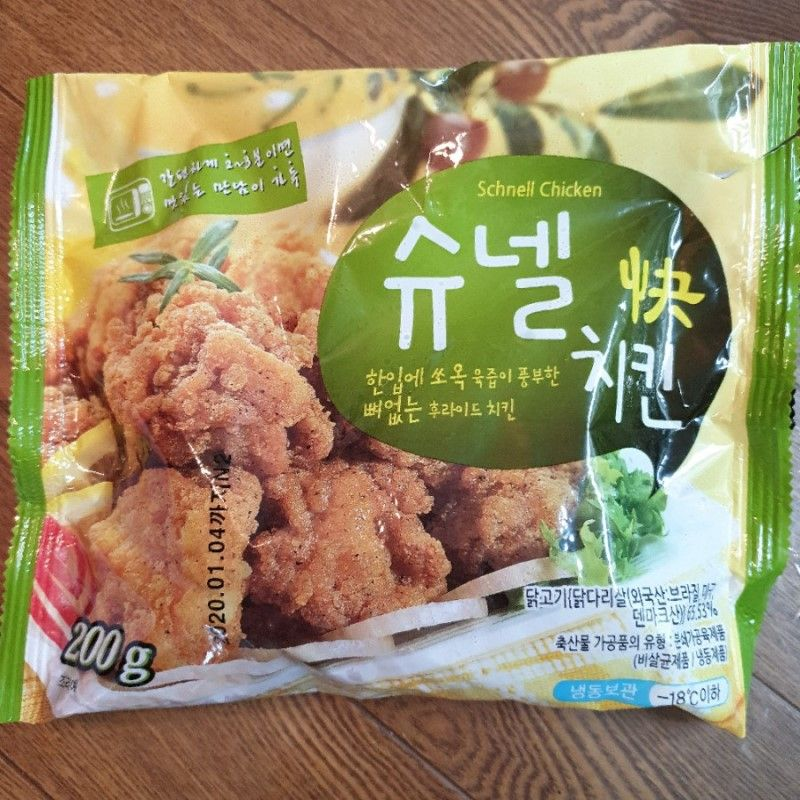
\includegraphics[width=0.3\textwidth]{problems/image/sunel_real.jpeg}
    \caption{슈넬치킨을 먹는 것이 군생활의 낙인 말년 병장 선우는 나쁜 짓을 저질렀다. 이에 선우는 군장을 메고 연병장을 도는 벌을 받게 되는데...}
\end{figure}

한 칸의 크기가 $1$이고 가장 왼쪽 위 좌표가 $(1,1)$, 가장 오른쪽 아래의 좌표가 $(N,M)$인 $N×M$ 크기의 연병장이 있다. 선우는 이 연병장의 가장자리를 돌아야 한다. 가장자리의 좌표는 $(i,1), (i,M)$ $(1\leq i\leq N)$ 과 $(1,j), (N,j)$ $(1\leq j\leq M)$로 표현할 수 있다. 가장자리를 제외한 연병장의 나머지 부분은 연병장의 안쪽으로 분류한다.

\begin{figure}[h]
    \centering
    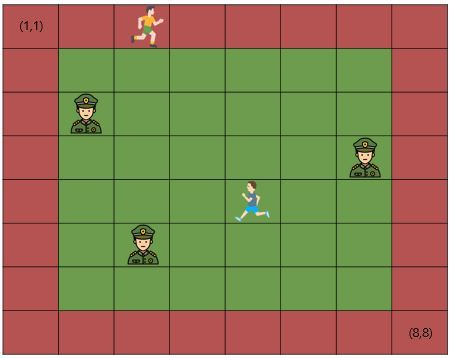
\includegraphics[width=0.4\textwidth]{problems/image/sunel_1.jpeg}
    \captionsetup{width=0.55\textwidth}
    \caption{[그림 1] $N=M=8$인 상황에서 선우와 상혁이의 상황이다. 빨간색 구역은 연병장의 가장자리, 초록색 구역은 연병장의 안쪽을 나타낸다.}
\end{figure}

선우의 맞후임 상혁이는 연병장의 안쪽에서 축구를 하던 중, 선우를 발견하고는 \textbf{슈넬치킨 랑데부}를 계획한다. 슈넬치킨 랑데부란 선우가 군생활 중 가장 좋아하는 음식인 슈넬치킨을 한 조각 주는 것으로, 상혁이와 선우가 연병장 격자 내의 같은 칸에 동시에 도착하는 경우에만 일어난다. 상혁이와 선우는 둘 다 초기에 칸의 중앙에 위치해 있다.

선우는 연병장의 가장자리 중 어딘가에서 출발해 1분마다 시계방향으로 이동하고 있고, 상혁이는 연병장의 안쪽에서 1분마다 인접한 칸으로 이동한다. 이때 연병장에는 상혁이와 같이 축구를 하던 간부들이 있기 때문에 간부가 있는 칸으로는 이동할 수 없다. 선우가 점점 지쳐가고 있기에 상혁이는 최대한 빨리 슈넬치킨 랑데부를 하고자 한다. 상혁이를 도와주자.

(어떤 두 칸이 변을 공유하는 경우 두 칸은 인접한 칸이라고 한다. 상혁이는 초기에 가장자리에 있지 않으며, 이동이 가능한 경우에는 연병장을 벗어나거나 가만히 있을 수 없다. 만약 이동이 불가능한 경우라면 그 자리에 머물러 있게 된다. 또한 간부는 초기 위치에서 움직이지 않는다.)

\newpage

\subsection*{입력}

첫째 줄에 $N$과 $M$이 주어진다. $(3\leq N,M\leq 1\,000)$

둘째 줄부터 $N$줄에 걸쳐 연병장에 대한 정보가 연병장 가장 위쪽 행의 정보부터 차례대로 각각 길이 $M$의 문자열로 주어진다.
여기서 \texttt{\color{red}A}는 상혁이, \texttt{\color{red}B}는 선우, \texttt{\color{red}G}는 간부, \texttt{\color{red}.}은 빈칸을 의미한다.

선우의 초기 위치는 가장자리임이, 간부와 상혁이의 초기 위치는 연병장의 안쪽임이 보장된다.

\subsection*{출력}

슈넬치킨 랑데부가 일어나기 위한 최소 시간을 출력한다.

만약 일어날 수 없다면 $-1$을 출력한다.

\subsection*{예제}

\begin{table}[h]
% \centering
\renewcommand{\arraystretch}{1.5}
\begin{tabular}{|L{8.2cm}|L{8.2cm}|}
\hline
\multicolumn{1}{|c|}{\textbf{standard input}} & \multicolumn{1}{c|}{\textbf{standard output}} \\ \hline\hline
% 적절한 예제를 입력하면 됩니다.
\texttt{3 3} & \texttt{1}\\ 
\texttt{B..} & \\ 
\texttt{.A.} & \\ 
\texttt{...} & \\
\hline

\texttt{3 3} & \texttt{-1}\\ 
\texttt{.B.} & \\ 
\texttt{.A.} & \\ 
\texttt{...} & \\
\hline

\texttt{7 10} & \texttt{8}\\ 
\texttt{...B......} & \\ 
\texttt{.......GG.} & \\ 
\texttt{....G.....} & \\
\texttt{..GGAGG...} & \\
\texttt{.G......G.} & \\
\texttt{..GGGGG...} & \\
\texttt{..........} & \\
\hline

\end{tabular}
\end{table}

\subsection*{노트}

\begin{itemize}
    \item 슈넬치킨 : 군 편의점 개념인 PX에서 파는 냉동 치킨 상품입니다.
    \item 연병장 : 단련할 련(鍊), 병사 병(兵), 마당 장(場) 입니다. 운동장의 개념과 비슷합니다.
    \item 군장 : 군인이 전투력을 유지하기 위해 장구를 휴대하는 방법 및 그에 쓰이는 장구를 뜻합니다.
    \item 간부 : 기관이나 조직체 따위의 중심이 되는 자리에서 책임을 맡거나 지도하는 사람을 말합니다.
    \item 문제에 등장하는 선우 : 사실 의경 출신이며, 수경 만기 전역을 하였습니다.
\end{itemize}
